\begin{surferPage}{Barth-flaten av sjette grad med 30 cusper} 
Etter at Wolf Barth hadde konstruert flaten av sjette grad med det maksimale antallet av $65$ singulariteter (se en annen flate i dette galleriet), og to av doktorgradsstudentene hans også hadde konstruert verdensrekordflater av høyere grad, begynte Barth å undersøke hvor mange cusper flater av en gitt grad maksimalt kan ha.  

   Barth-flaten av sjette grad med 65 singulariteter av type $A_1^{+-}$ (doble kjegler) kan tilpasses cusper. Det gir 30 cusper: 
   
    \[P_6 - \alpha \cdot K^3=0,\]
  hvor $P_6$ er de samme symmetriplanene som for ikosaedret og for den andre Barth-flaten av sjette grad, og hvor $K$ er ligningen til en kuleoverflate:
    \vspace*{-0.4em}
    \begin{center}
      \begin{tabular}{c@{\ }c@{\ }c@{\ }c}
        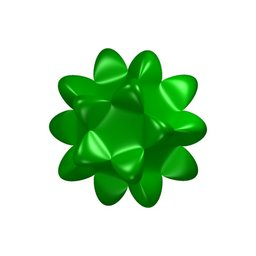
\includegraphics[height=1.2cm]{./../../common/images/barthsextic_30A2}
        &
        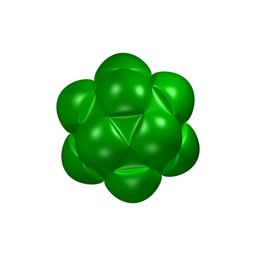
\includegraphics[height=1.2cm]{./../../common/images/barthsextic_30A2_3}
        &
        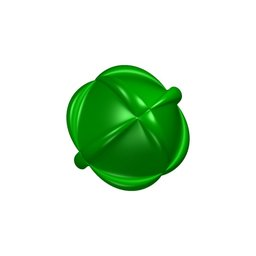
\includegraphics[height=1.2cm]{./../../common/images/barthsextic_30A2_5}
        &
        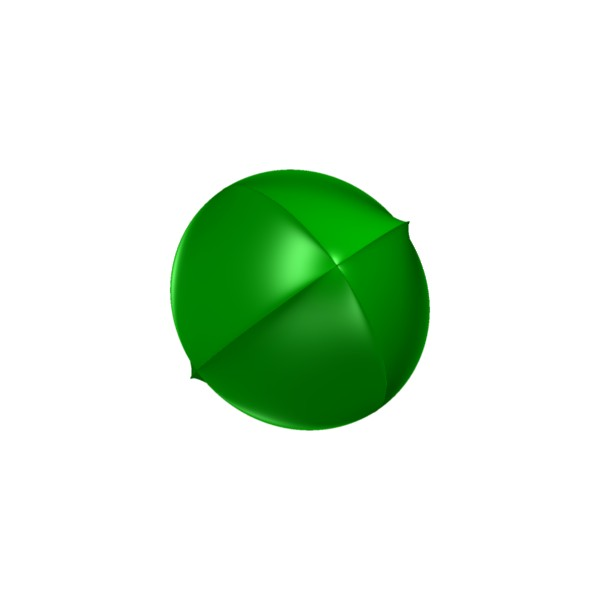
\includegraphics[height=1.2cm]{./../../common/images/barthsextic_30A2_6}
      \end{tabular}
    \end{center}    
    \vspace*{-0.3em}
   Dette er den gjeldende verdensrekorden for det maksimale antallet av reelle cusper på flater av sjette grad. For komplekse cusper er tallet $36$.
\end{surferPage}
